% Spiego l'idea
% chi è stato
% e perchè
% come funziona

Parasitic computing\footnote{In this thesis we are not covering, neither
we are interested in, the ethical or moral implication of using this technique.}
is a technique that, using some exploits and ad-hoc code, allow a \emph{malicious}
user to use the computational power of the \emph{victim} computer without this
being aware. As one can notice parassitic compiting has a strong relationship
with \emph{distributed computing}, in fact is a specialization of the general
class of \emph{voluntary computing}, where the user is unaware of
the execution\footnote{In \emph{voluntary computing} the user can be unaware
of the actual code they are executing, but they are aware of the execution.}.\\

This approach was first proposed by \cite{barabasi2001parasitic} to solve the
NP-complete 3-SAT problem using the existing TCP/IP protocol stack and its error
handling routines. The satisfiability problems or "SAT" involves finding a
solution to a boolean equation that satisfies a number of logical clauses. For
example, $(x_1 \oplus x_2) \land (x_2 \land x_3 )$ in principle has $2^3$ potential
solutions, but it is satisfied only by the solution: $x_1=1, x_2=0, x_3=1$.
Problems problem like the one in the example are known as 2-SAT problem because
each clause, shown in parentheses, involves two variables. The more difficult
3-SAT problem is known to be NP-complete, which in practice means that there is
no known polynomial-time algorithm which solves it.\\
\begin{figure}[htb]
    \centering
    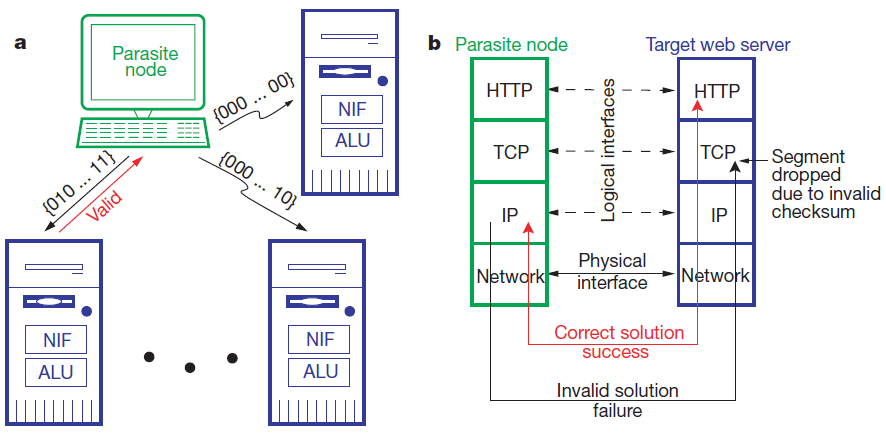
\includegraphics[width=\columnwidth]{parasitic}
    \caption{Schematic diagram of the parasitic computer solving the 3-SAT
    problem.}
    \label{fig:parasitic}
\end{figure}

The approach proposed in the paper was to perform a brute force attack to guess
the right solution of a 3-SAT problem using a parallel apprach as depicted in
\autoref{fig:parasitic}. The parasite node creates $2^n$ specially constructed
messages designed to evaluate a potential solution. These messages are sent to
many target servers throughout the Internet. After receiving the message, the
target server verifies the data integrity of the TCP segment by calculating a
TCP checksum. The construction of the message ensures that the TCP checksum fails
for all messages containing an invalid solution to the posed SAT problem. Thus,
a message that passes the TCP checksum contains a correct solution. The target
server will respond to each message it receives (even if it does not understand
the request). As a result, all messages containing invalid solutions are dropped
in the TCP layer. Only a message which encodes a valid solution \emph{reaches}
the target server, which sends a response to the \emph{request} it received.\\

This approach may seem wrong or at leat not right, with respect to the user, but
if one think about it notice how we are always making computation without even
knowing. \ac{GWAP} or application like \href{reCAPTCHA}{http://www.google.com/recaptcha}
are examples of involuntary human computation (as in \autoref{tab:matrix}). So
thay are using the same technique to perform a sort of \emph{parasitic human
computing} without complainig about the user will.\\

To avoid the ethic implication of doing \emph{parasitic computing} a hybrid
approach (parasitic/voluntary) can be used. If the user give the permission to
run computation on its computer exchange of a return of any type, then we are
able to score the best on both approaches. A similar solution was proposed in
\cite{karame2011pay}.
In this paper they propose a microcomputations as micropayments in web-based
services. Their solution is to give the user access to online contents (such as
newspaper, video, etc.) after performing small \js{} computation.

% Usando lo stesso approccio ma in js

The main drawback of distributed computing is the portability and distribution.
The installation of some kind of client to execute the code can be seen as a problem for some
user, as an example some users simply cannot install software on their workstation, due to security
restriction or missing disk space. The other problem is distribution, the main purpose of these
frameworks is to perform massive parallel computation, but for the computation to be really 
massive we need a lot of volunteers that installed the client on their pc and are online to execute
the code.

\paragraph{Parasitic \js{}} can lead to a solution of these problems using a widespread
and standard technologies. Using the Web as the distribution platform the audiance can scale
rapidly from to thousands to hundred thousands of users. Regarding the need of third part software
installation and security issues, using \js{} these problems are avoided, because all the code the browsers
runs is executed into a sandboxed execution environment so it cannot harm the users pc. The same stands
for the portability of the code, bacause almost all bowsers\footnote{\emph{**COUGH**} IE \emph{**COUGH**}} support
\js{} with all the HTML5 features (see~\ref{sec:bg:web:html5}), so the porting of the code
is guaranteed on every system that can run a browser.